\section{Introduction}
\label{sec:introduction}

\begin{figure}% [ht]
    \centering
    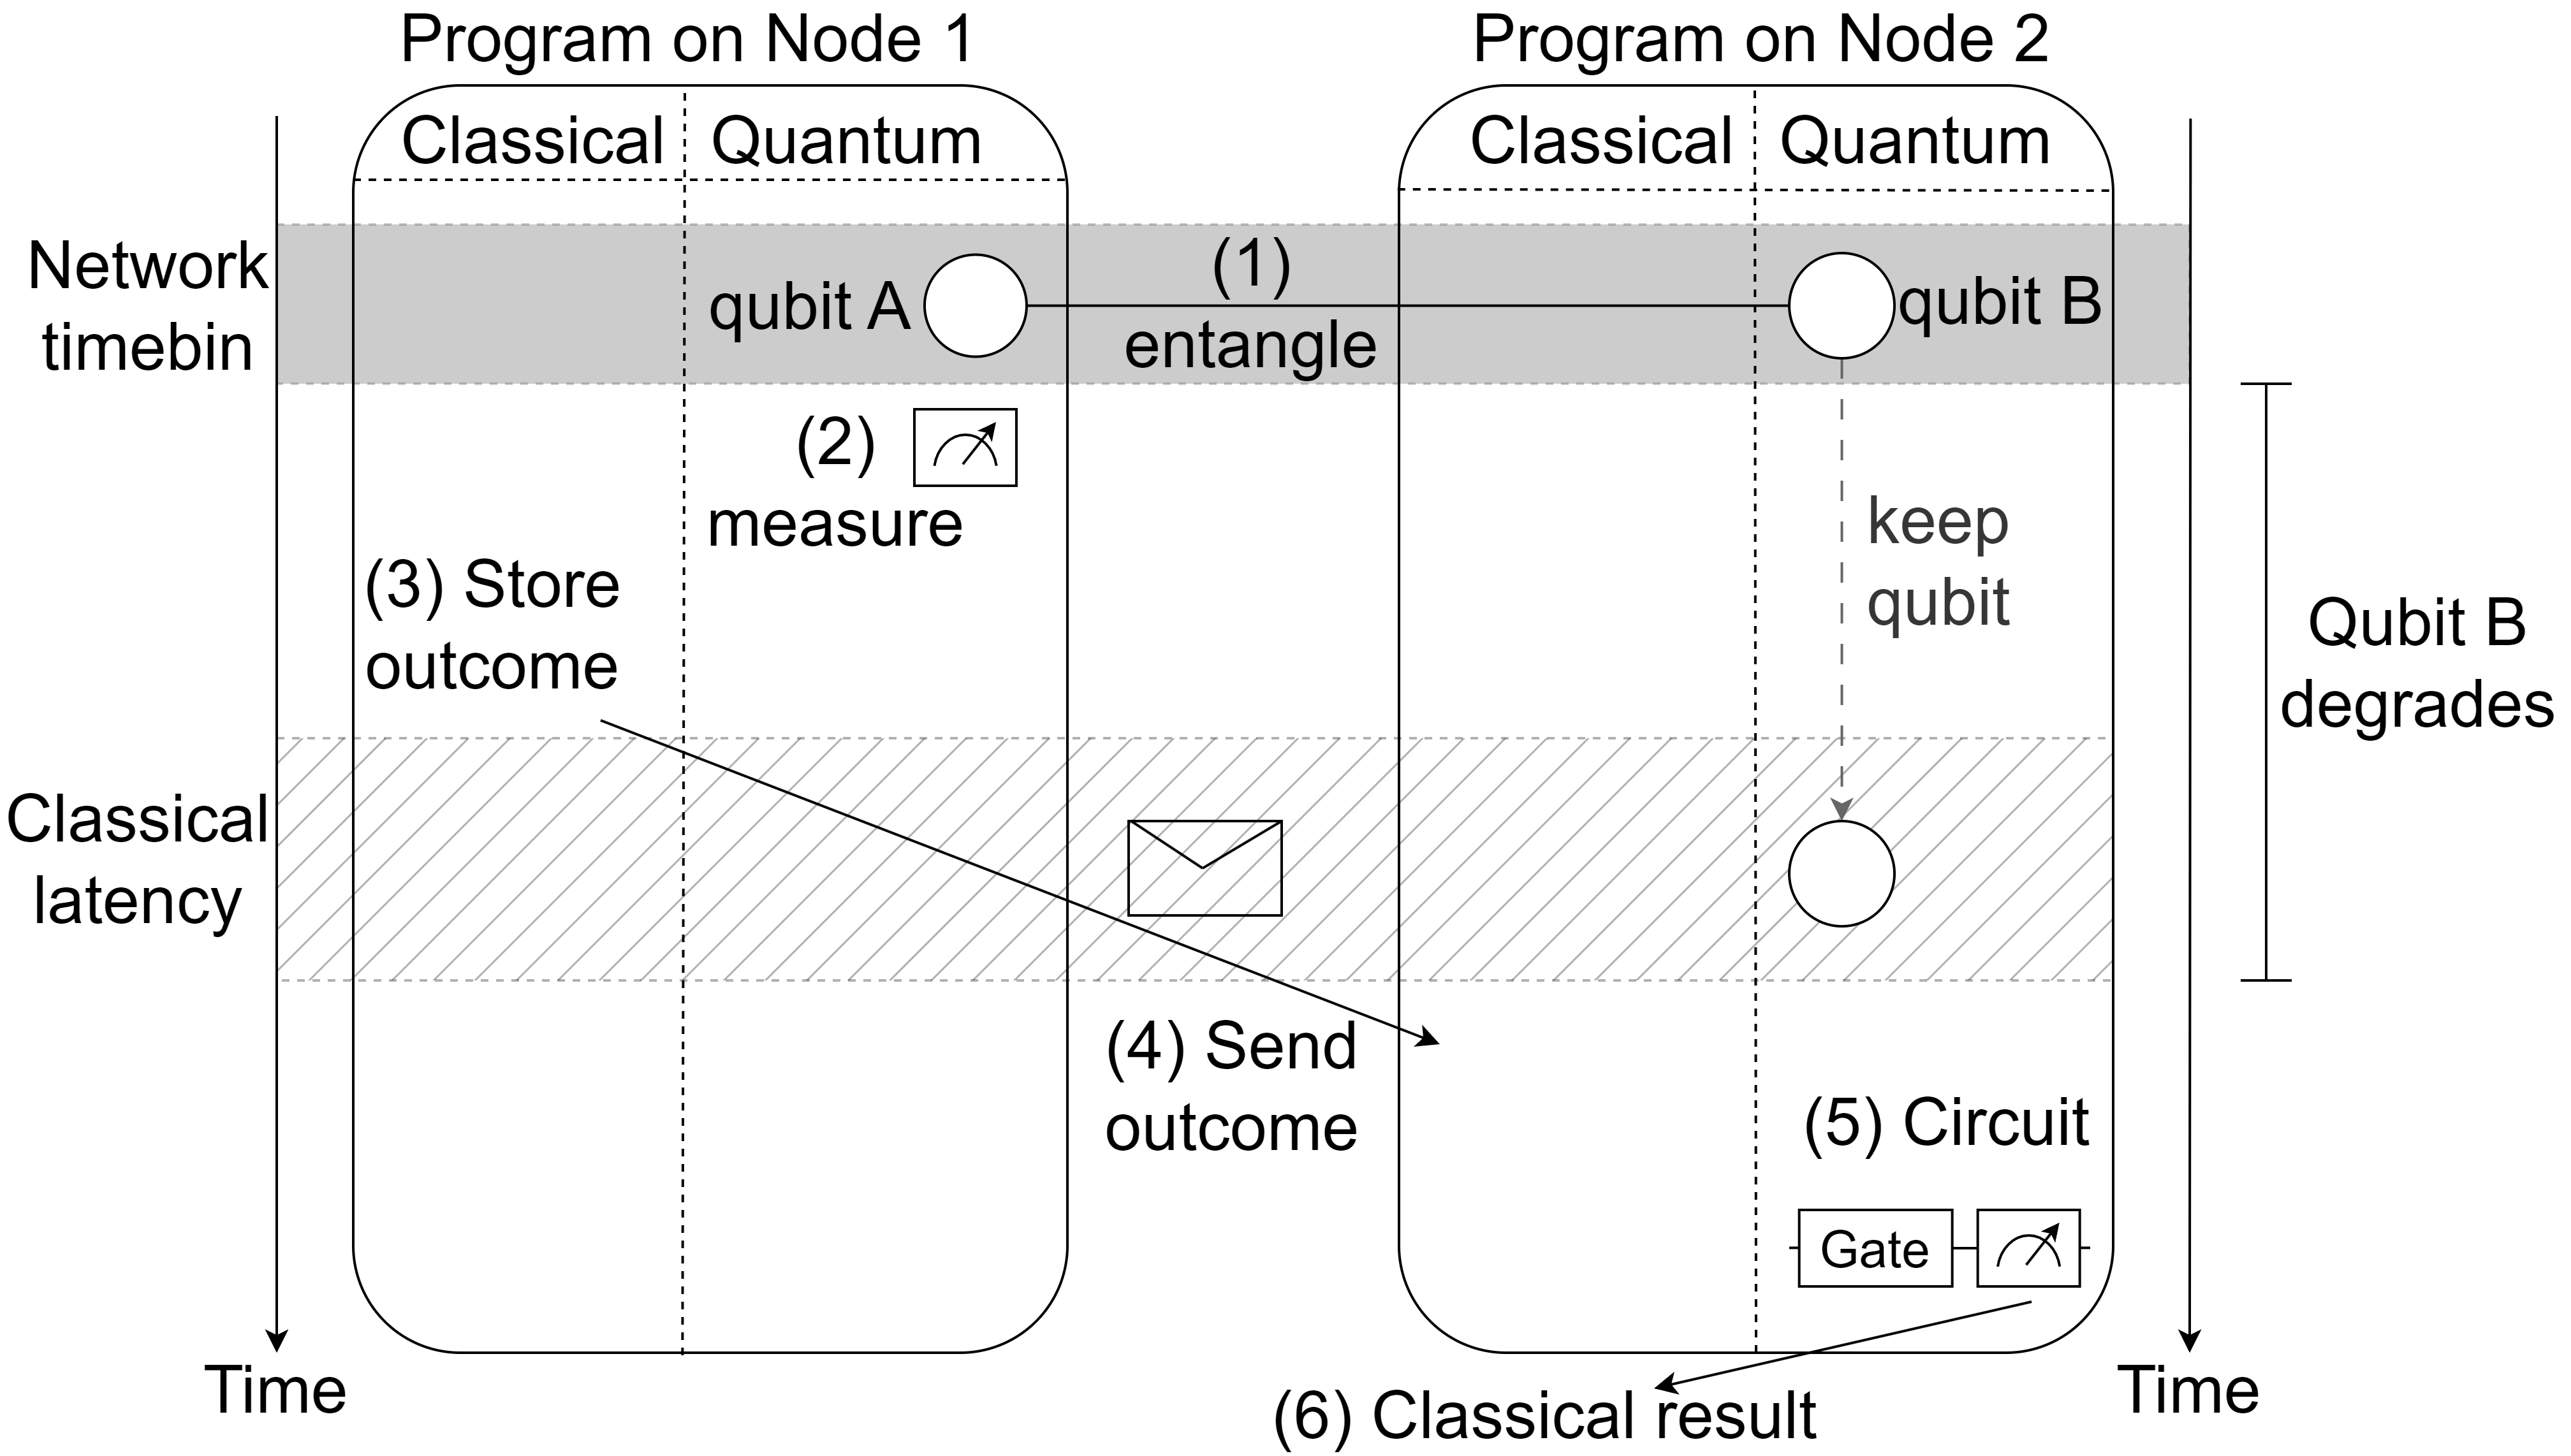
\includegraphics[scale=0.35]{figures/qoala/program_illustration.png}
    \caption{Example application consisting of two hybrid classical-quantum programs (on Nodes 1 and 2) including
        (1) Entanglement generation between two qubits (circles) in a synchronized time slot (defined by  network controller).
        (2) A local measurement of qubit A at Node 1 resulting in a classical outcome bit (destroying the qubit)
        (4) Communication of the classical bit from Node 1 to Node 2 (taking non-deterministic time)
        (5) Execution of a quantum circuit on qubit B at Node 2 depending on the classical bit. The quality of qubit B has degraded during the time elapsed since (1). 
        (6) Node 2 measures qubit B and outputs the classical result.
    }
    \label{fig:program_illustration}
\end{figure}


\todo{Merge with intro chapter}
Advances in quantum computing and quantum communication technologies are paving the way for a \textit{quantum internet}~\cite{wehner2018quantum, kimble2008quantum}, where quantum applications are executed across multiple network nodes.
Examples of such applications include quantum key distribution (QKD)~\cite{bennett2014quantum, ekert1991quantum} and blind quantum computation (BQC) \cite{broadbent2009universal, arrighi2006blind} from a client to a quantum cloud server.
A multi-node quantum internet application is partitioned into separate single-node \textit{programs} (e.g. a client program and a server program in BQC) that run concurrently on different network nodes. To support security sensitive applications, each program performs local classical and quantum computations on its own private node, and programs interact with each other only via classical message passing and entanglement generation. This is in sharp contrast to distributed quantum computing (see e.g.~\cite{cacciapuoti2019quantum}), where all nodes can be accessed and controlled by a single program. 

The single-node programs that constitute a quantum internet application are hybrid in nature (see Fig~\ref{fig:program_illustration}):
First, they contain quantum operations, such as local quantum gates and measurements (e.g. to perform a server computation in BQC), and entanglement generation (e.g. to produce key in QKD). Entanglement is a special property of two quantum bits (qubits) that forms a key resource for quantum internet applications. 
All quantum operations are executed on quantum processors that can store, manipulate and measure quantum information, where small networks including such processors have been realized using different quantum hardware platforms including, for example,  Nitrogen-Vacancy (NV) centers in diamond~\cite{pompili2021realization}, and Ion Traps~\cite{krutyanskiy2023entanglement}.
Second, programs need to perform classical operations, such as message passing (e.g., a BQC client program sending desired measurement bases to the BQC server), and local classical processing (e.g., post-processing measurement outcomes in QKD).

Realizing the execution of quantum internet applications presents unique challenges (see Section~\ref{sec:design_considerations}): 
First, a program for a quantum internet application is not merely a hybrid of classical and quantum code segments; these segments are also highly \textit{interactive}: classical and quantum code may run concurrently, communicating and influencing each other.
E.g., a quantum circuit may "pause" halfway, keeping quantum states in memory, and wait for a value from a classical segment (e.g. a classical message from a remote node) before continuing.
Quantum memories have limited lifetimes, meaning qubits are subject to decoherence, degrading their quality over time. This introduces the need 
control the joint schedule of the classical and quantum segments of the program to reach desired levels of application performance.

Second, a compiler should be able to optimize the whole program including both classical and quantum code, as well as to provide information that can be used in our architecture to align and inform scheduling decisions. 

Finally, we are faced with a mix of time scales:
on the one hand, entanglement generation requires a very precise network schedule that is agreed ahead of time between the network nodes~\cite{dahlberg2019link}. On the other hand, classical messages are exchanged asynchronously between the nodes without guaranteed message delivery times. This motivates an architecture in which different segments of the system may operate at different levels of timing precision. 

\subsection{Main contributions}
We propose the first architecture, Qoala, that addresses these challenges. Qoala is an execution environment tailored to programmable quantum internet nodes, accommodating the \textbf{hybrid, interactive, networked, and asynchronous nature} of quantum internet applications. 

\textbf{Unified program format for hybrid-classical quantum programs:}
Qoala defines a unified program format for executables, encompassing classical and quantum (networked and local) code, and defining basic blocks.
This paves the way for a joint optimization of the classical and quantum code by a compiler.
% The program format is also made such that it can be the output of a compiler, making use of basic blocks.

\textbf{Runtime representation allowing scheduling:} Qoala separates the static unified program format from a runtime representation consisting of \textit{tasks}. 
This paves the way to design and implement algorithms for scheduling the quantum program in order to meet deadlines imposed by decoherence of the quantum memory.  
To provide advice to the scheduler on deadlines to achieve a desired program performance, programs can specify advice for timing and prioritization depending 
on the quantum hardware capabilities of the node. 
The separation of a static program from its runtime tasks also allows for the programmer to define asynchronous code segments, the execution of which is decided by the scheduler alone.
This is the first architecture that allows for effective scheduling control of hybrid interactive classical-quantum programs, thus addressing a critical issues in the successful execution of quantum internet applications.

\textbf{Integration with quantum network stack:}
Qoala integrates with an existing quantum network stack~\cite{dahlberg2019link} implemented on NV centers in diamond~\cite{pompili2022experimental} for realizing entanglement generation between nodes. This opens the door for Qoala to be implemented on such networks.

\textbf{Implementation in hardware validated simulation:} We implement the proposed architecture as a \textbf{modular and composable simulator}, which enables the evaluation of different execution strategies and techniques.
The simulation is validated against real-world quantum hardware implementations, opening the door to understand performance tradeoffs and requirements for Qoala's implementation. Specifically, the simulator allows 
configuring different hardware parameters, latencies, and software component organizations, to evaluate implementation choices of Qoala in simulation. 

Using the implementation we demonstrate the effectiveness and feasibility of our proposed architecture on different types of quantum hardware, including its ability to schedule and multitask applications using a number of existing scheduling methods (EDF, FCFS).
We continue to examine tradeoffs in the classical and quantum performance metrics of using different types of scheduling approaches. 
We examine Qoala's improvement over NetQASM~\cite{dahlberg2022netqasm} in enabling hybrid classical-quantum compilation possibilities. 
Finally, we study trends in application performance when varying the amount of concurrency, and examine the impact of a network schedule for entanglement generation on the performance of Qoala.

We highlight the role of Qoala in opening the door for computer science research. We make our simulator available as open source~\cite{qoala2023simulator}, paving the way for computer scientists to conduct further research, e.g., into the design of compilers, or schedulers that can readily be tested using the simulator. 

The remainder of this paper is structured as follows. Section~\ref{sec:related_work} compares our work to related studies. In Section~\ref{sec:design_considerations} we explain important context and terminology, followed by considerations that we used to design our architecture (Section~\ref{qoala:sec:architecture}). Section~\ref{sec:implementation} discusses our implementation and Section~\ref{qoala:sec:evaluation} provides evaluation results using this implementation. We conclude and give suggestions on future work (Section~\ref{sec:conclusion}).

